\documentclass[notheorems,hyperref={bookmarks=true}]{beamer}
\usepackage[framesassubsections]{beamerprosper}
\hypersetup{pdfpagemode=FullScreen}
\usepackage[utf8]{vietnam}
\usepackage{mdframed}
\usepackage[english]{babel}
\usepackage{ulem} %for underlying+
\usepackage{pifont} %for creating dingautolist
\usepackage[mathscr]{eucal}
\usepackage{amsfonts,amsmath, amsthm, amssymb,amsxtra,latexsym,amscd,graphics,graphpap}
\usepackage{indentfirst}
\usepackage{rotating}
\usepackage{graphicx}
\usepackage{amsbsy}
\usepackage{epsfig}
\usepackage{natbib}
\usepackage{cases} 

\usepackage{pdfpages}
\usepackage{multicol}
\usepackage{hyperref}
\usepackage{subfigure}
\usepackage{multimedia}
\usepackage{boxedminipage}
\usepackage{tikz}
\usepackage{nicefrac}
\setbeamertemplate{theorems}[numbered] % Đánh số định lý.
\usetheme{Boadilla} % puts title, section, etc on top

\usecolortheme{rose} 
\usefonttheme[onlylarge]{structurebold}
\usefonttheme{professionalfonts}
\setbeamercolor{title}{fg=red!80!black,bg=blue!20!white}
\setbeamertemplate{section in head/foot shaded}[default][20]
\setbeamertemplate{subsection in head/foot shaded}[default][20]
\setbeamertemplate{navigation symbols}{}
\setbeamertemplate{blocks}[rounded][shadow=true]
\setbeamerfont{small}{size=\small}
\setbeamerfont{footnote}{size=\footnotesize}
\setbeamerfont{script}{size=\scriptsize}
\setbeamerfont{tiny}{size=\tiny}

\theoremstyle{plain}
\newcommand{\thedefinition}{\arabic{section}.\arabic{definition}}
\newcommand{\thelemma}{\arabic{section}.\arabic{lemma}}
\newcommand{\thetheorem}{\arabic{section}.\arabic{theorem}}
\renewcommand{\thetable}{\Roman{table}}

\mode<presentation>
\setbeamertemplate{navigation symbols}{} 

\usepackage{wrapfig}
\usepackage{multicol}
%\setbeamertemplate{footline}{\raisebox{-2.2ex}{\pgfuseimage{logo.png}}}

\title[{\makebox[.15\paperwidth]{VARMAX \& LSTM in Air Quality prediction}}]{Mô hình VARMAX và LSTM \\ trong dự báo chất lượng không khí} 
\author[Nhóm 16]{Nhóm 16
\\Phạm Thị Hoa - 20195874\\
Lê Thanh Thảo - 20195919\\
Phạm Thu Trang - 20195931\\
\\
                Giảng viên hướng dẫn: TS. Nguyễn Thị Ngọc Anh} 
\date{Hanoi, 3/2023}

\renewcommand{\sfdefault}{cmss}
\renewcommand{\rmdefault}{cmr}
\renewcommand{\ttdefault}{cmtt}
\numberwithin{equation}{section}
\usepackage{array}
\usepackage{ragged2e}
\justifying
\usepackage{blindtext}
\usepackage{geometry}
 \geometry{
right = 5.5mm
 }
\renewcommand{\baselinestretch}{1.15}
\setlength{\parindent}{1.5em}
%\setlength{\parskip}{1em}
\DeclareMathOperator*{\argmin}{arg\,min}
\newtheorem{prop}{Proposition}
\usepackage{amsmath}
\newtheorem{definition}{Definition}
\newtheorem{theorem}{Theorem}
\newtheorem{corollary}{Corollary}
\newtheorem{hypothesis}{Hypothesis}
\usepackage{esvect}
\usepackage{booktabs}
\usepackage{multirow}

\begin{document}
	\begin{footnotesize}
		\begin{frame}
			\frametitle{}
			\maketitle
			%	\begin{block}
			%	\titlepage
			%	\end{block}
		\end{frame}
		
		\AtBeginSection[] % Do nothing for \section*
		{
			\begin{frame}<beamer>
				\frametitle{Outline}
				\tableofcontents[currentsection, currentsubsection]
			\end{frame}
		}
	\begin{frame}{Outline}
	    \tableofcontents
	\end{frame}	
 
	\section{Giới thiệu bài toán}
   % \begin{frame}{Tổng quan tình hình nghiên cứu}
        %\begin{itemize}
            %\item Ariyo, A. A., Adewumi, A. O., & Ayo, C. K. (2014). Stock Price Prediction Using the ARIMA Model. 2014 UKSim-AMSS 16th International Conference on Computer Modelling and Simulation. 
            %\item Ma, Q. (2020). Comparison of ARIMA, ANN and LSTM for Stock Price Prediction. E3S Web of Conferences, 218, 01026. 
            %\item Siami-Namini, S., Tavakoli, N., & Siami Namin, A. (2018). A Comparison of ARIMA and LSTM in Forecasting Time Series. 2018 17th IEEE International Conference on Machine Learning and Applications (ICMLA). 
            %\item ...
        %\end{itemize}
    %\end{frame}
    
    \begin{frame}{Giới thiệu bài toán}
    \begin{itemize}
        \item Sử dụng hai mô hình VARMAX và LSTM dự đoán chất lượng không khí.
        \item Đối tượng nghiên cứu: các chỉ số ảnh hưởng đến chất lượng không khí trong một khu vực: nhiệt độ, độ ẩm, lượng bụi mịn PM10, PM 2.5, nồng độ CO, SO2, NO... trong không khí
        \item Phạm vi nghiên cứu: từ ngày 14/4/2015 tới ngày 5/9/2019.
    \end{itemize}
    \end{frame}
    
    \section{Mô hình VARMAX}       
    \begin{frame}{Frame Title}
	\frametitle{Mô hình VARIMAX}
    Mô hình VARMAX gồm 3 thành phần chính:
    \begin{itemize}
		\item Vector Auto regression (VAR)
		\item Moving average (MA)
		\item Exogenous variable (X) 
		\end{itemize}
    \end{frame}
    
    \begin{frame}{Frame Title}
	\frametitle{Mô hình VARIMAX}
   Mô hình toán học của VARMAX được định nghĩa như sau:
\begin{equation}
    y_t = v + A_1y_{t-1} + \cdots + A_py_{t-p} + Bx_t + \epsilon_t + M_1\epsilon_{t-1} + \cdots + M_q\epsilon_{t-q}
\end{equation}
trong đó: 
\begin{itemize}
    \item \textbf{$y_t$} là một vector của các giá trị hiện tại và các giá trị $y$ khác là các giá trị trễ.
    \item \textbf{$A_s$} là các hệ số tự tương quan: đối với mỗi độ trễ, chúng là một vector có cùng độ dài với số lượng chuỗi thời gian.
    \item \textbf{$M_s$} là vector của các hệ số của các sai số mô hình trễ. Chúng đại diện cho phần trung bình cộng của mô hình.
\end{itemize}
    \end{frame}
   
    \section{Mô hình LSTM}
    \begin{frame}{Mô hình Long Short-term Memory}
    \begin{itemize}
        \item Mạng bộ nhớ dài-ngắn (Long Short Term Memory networks), thường được gọi là LSTM - là một phiên bản mở rộng của mạng thần kinh hồi quy (RNN) nhân tạo được sử dụng trong lĩnh vực học sâu.
        \item LSTM được giới thiệu bởi \textbf{Hochreiter \& Schmidhuber}  vào năm 1997.
        \item LSTM được thiết kế để giải quyết các bài toán về phụ thuộc xa (long-term dependency) trong mạng RNN do bị ảnh hưởng bởi vấn đề gradient biến mất.
    \end{itemize}  
    \end{frame}

    \begin{frame}{Mô hình Long Short-term Memory}
    Một đơn vị LSTM thông thường bao gồm:
    \begin{itemize}
    \item \textbf{Tế bào (cell)}
    \item \textbf{Tầng cổng quên (forget gate)} 
    \item \textbf{Tầng cổng vào (input gate)} 
    \item \textbf{Tầng ổng ra (output gate)}
\end{itemize} 
    \end{frame}

    \begin{frame}{Trạng thái tế bào (Cell state)}
        \begin{figure}[H]
        \centering
        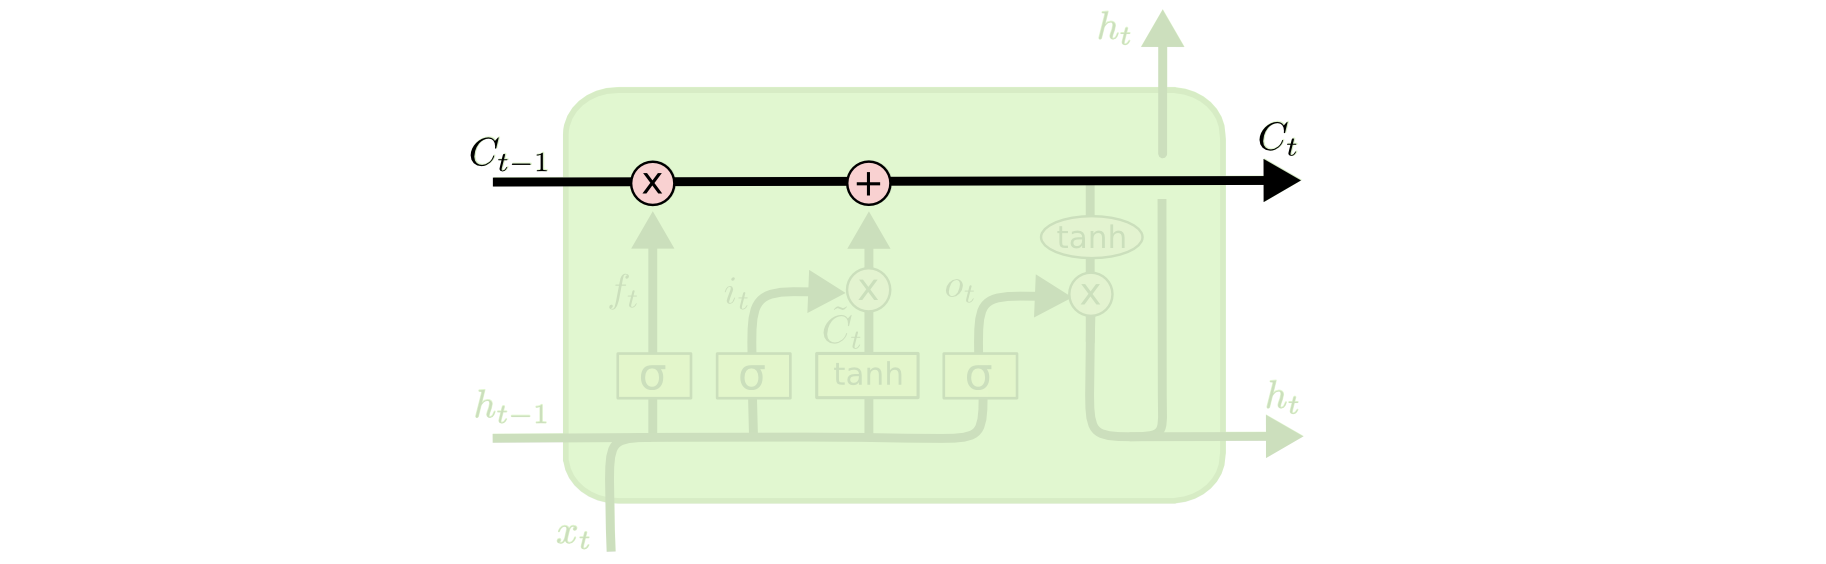
\includegraphics[width=1.2\textwidth]{figures/LSTM3-C-line.png}
        \caption{Cell state in LSTM.}
        \label{fig:cell_state}
        \end{figure}
        \par
    \end{frame}
    
    \begin{frame}{Kiến trúc bên trong LSTM}
        \begin{figure}[H]
        \centering
        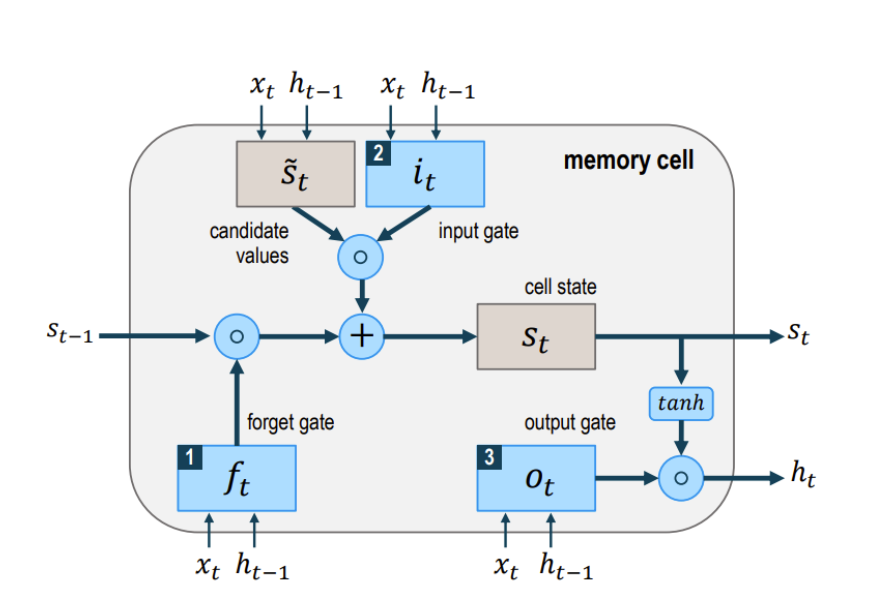
\includegraphics[width=0.8\textwidth]{figures/sodo.png}
        \caption{Sơ đồ biểu diễn kiến trúc bên trong của một tế bào LSTM.}
        \label{fig:cell_state}
        \end{figure}
        \par
    \end{frame}
    
\begin{frame}{Tầng cổng quên}
\begin{figure}[H]
\centering
	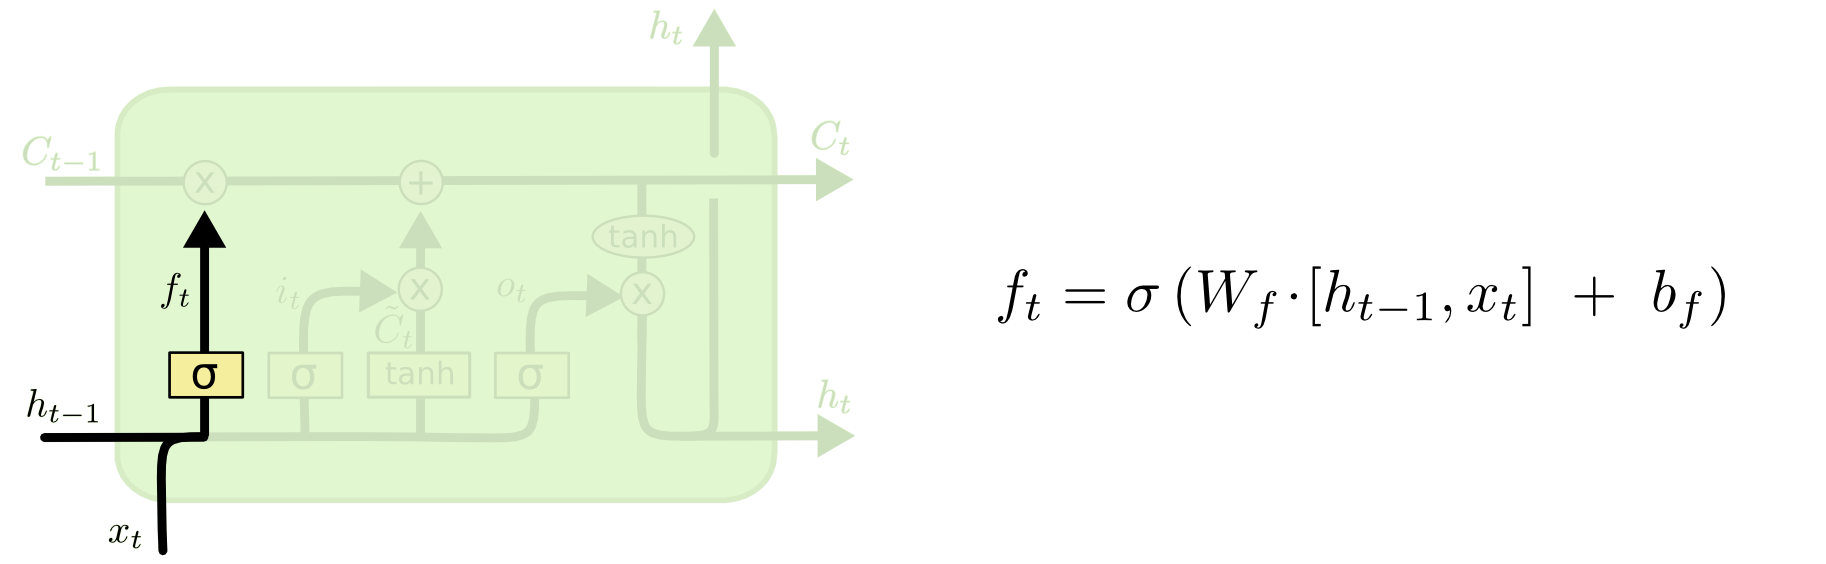
\includegraphics[width=\linewidth]{figures/LSTM3-focus-f.png}
	\caption{Tầng cổng quên.}
\end{figure}
\par Tầng cổng quên có nhiệm vụ loại bỏ những thông tin không cần thiết nhần được khỏi cell internal state.
\end{frame}

\begin{frame}{Tầng cổng vào}
\begin{figure}[H]
\centering
	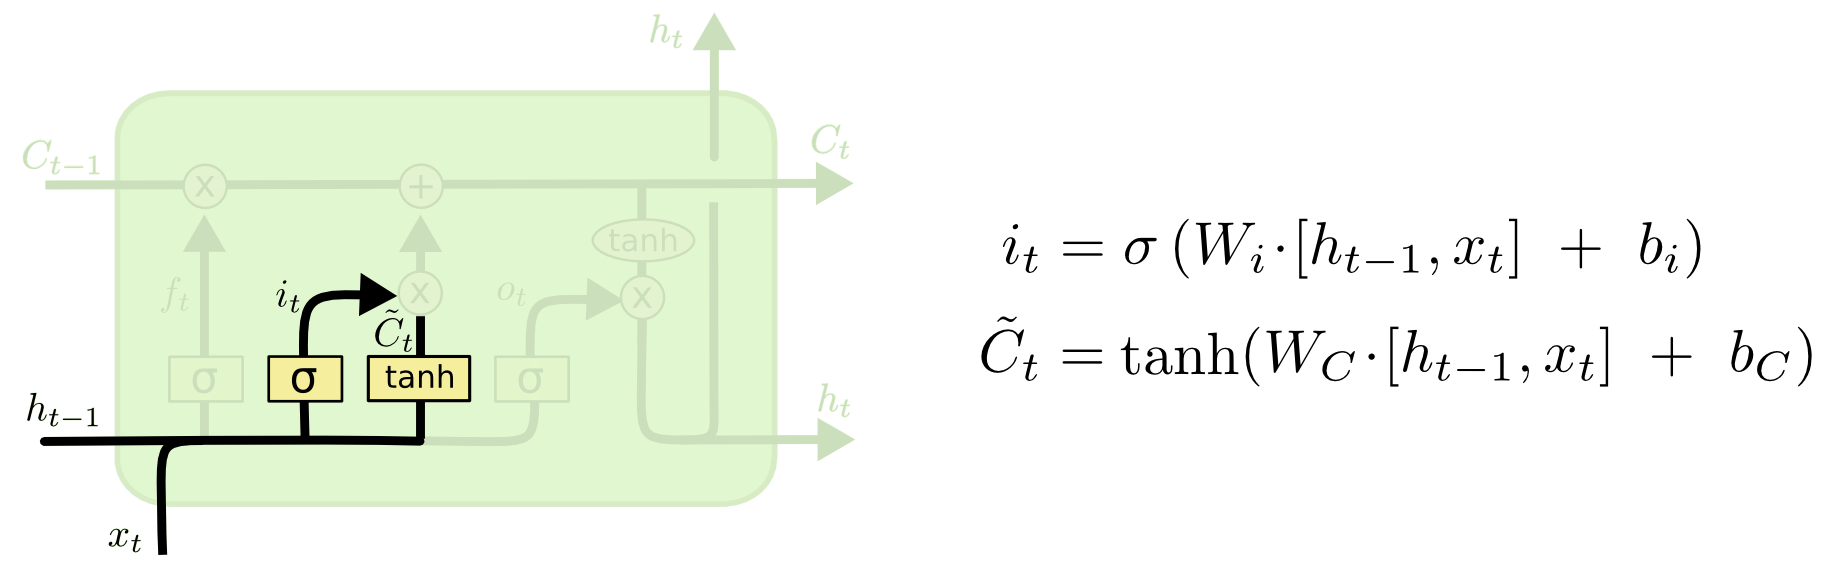
\includegraphics[width=\linewidth]{figures/LSTM3-focus-i.png}
	\caption{Tầng cổng vào.}
\end{figure}

\par Tầng cổng vào có nhiệm vụ chọn lọc những thông tin cần thiết nào được thêm vào cell internal state. 
\end{frame}

\begin{frame}{Cập nhật trạng thái tế bào}
\begin{figure}[H]
\centering
	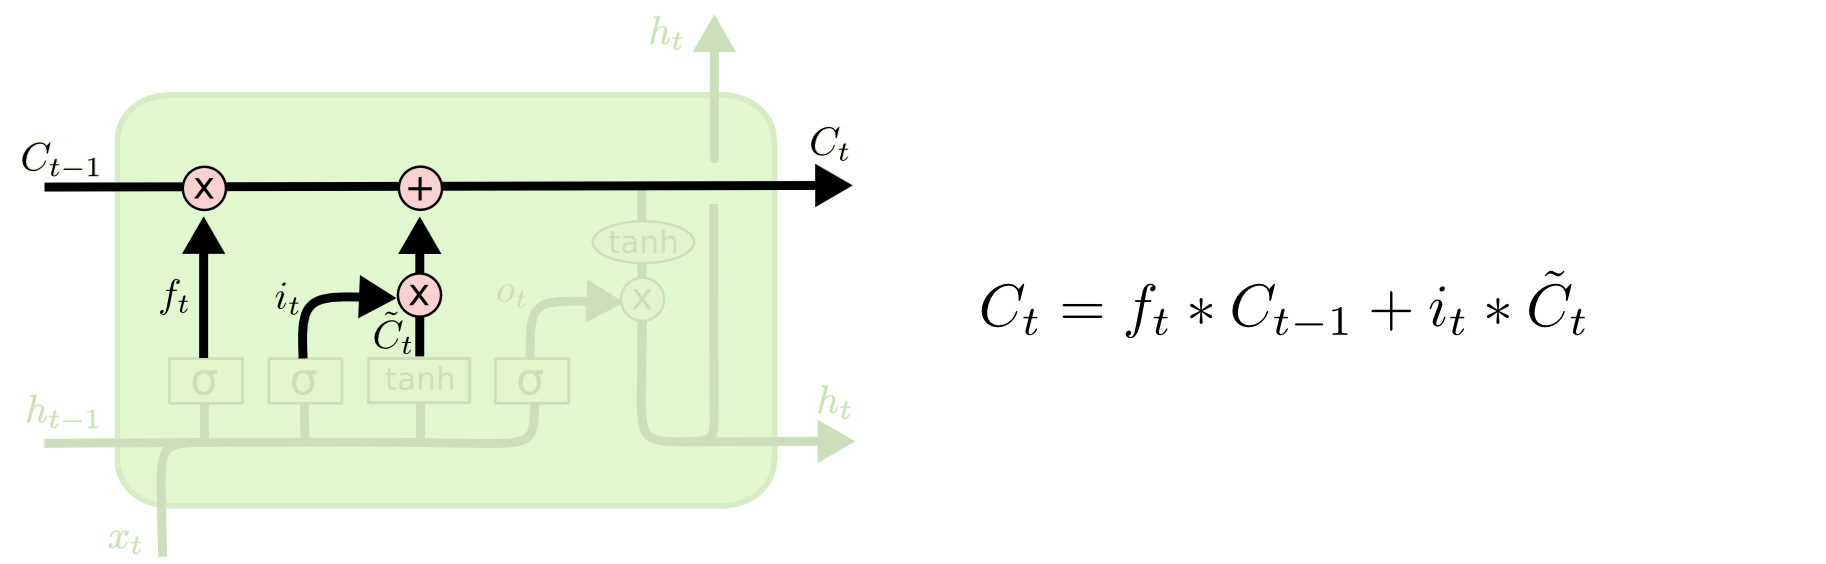
\includegraphics[width=\linewidth]{figures/LSTM3-focus-C.png}
	\caption{Cập nhật trạng thái tế bào.}
\end{figure}
\end{frame}
    \begin{frame}{Cổng ra}
\begin{figure}[H]
\centering
	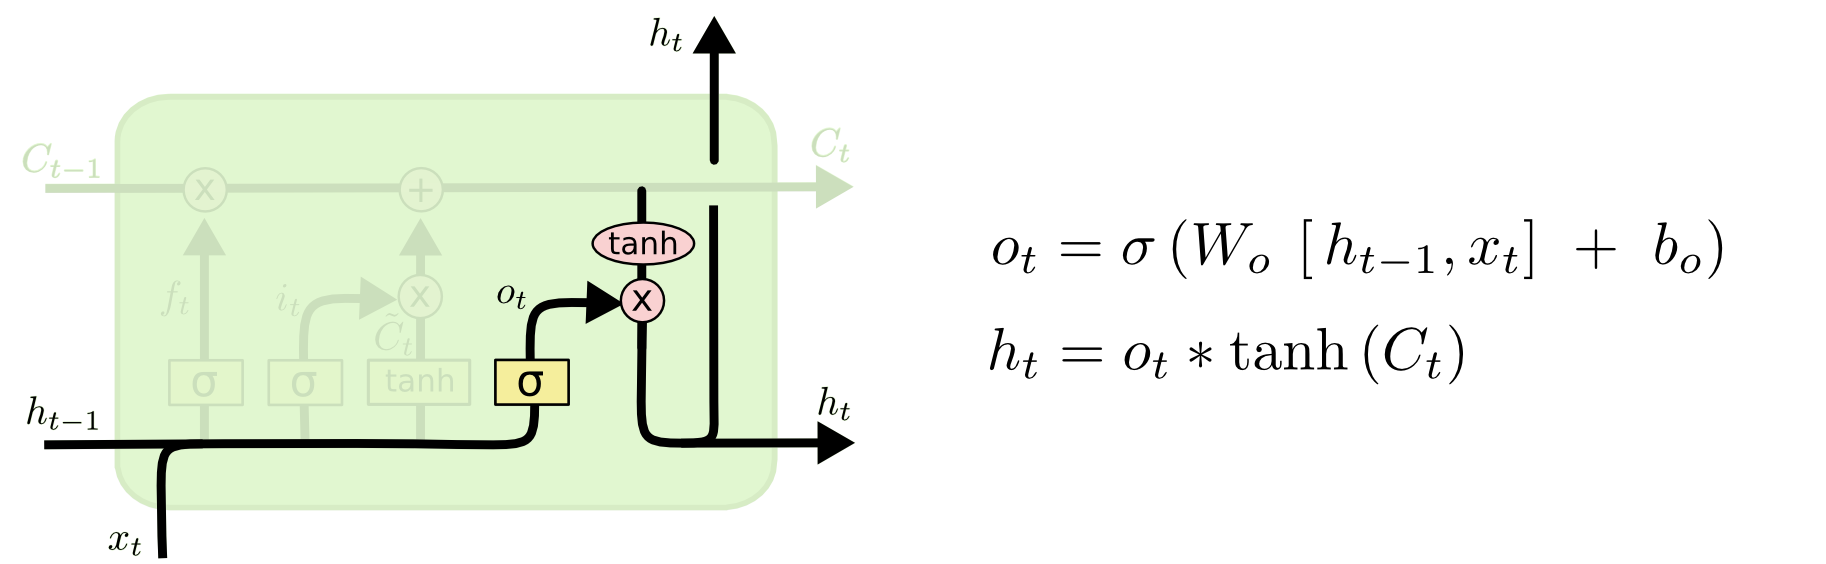
\includegraphics[width=\linewidth]{figures/LSTM3-focus-o.png}
	\caption{Cổng ra.}
\end{figure}
\par Tầng cổng ra có nhiệm vụ xác định những thông tin vào từ cell internal state được sử dụng như đầu ra.
    \end{frame}
    \section{Kết quả thực nghiệm}
    \begin{frame}{Mô tả bộ dữ liệu}
Để thực hiện dự đoán với hai mô hình  LSTM và VARMAX, chúng em sẽ thực nghiệm trên dữ liệu về chỉ số môi trường không khí.
\begin{itemize}
    \item Nguồn thu thập: Được cung cấp bởi giảng viên bộ môn
    \item Thời gian của dữ liệu: 142 ngày từ 7:00 14/4/2019 đến 6:00 5/9/2019 tính theo từng giờ.
    \item Kích thước dữ liệu: 556KB
    \item Giá trị cần dự đoán: mô hình dự đoán tất cả các giá trị trong bộ dữ liệu
\end{itemize}
    \end{frame}
        \begin{frame}{Mô tả bộ dữ liệu}
\begin{figure}[H]
    \centering
    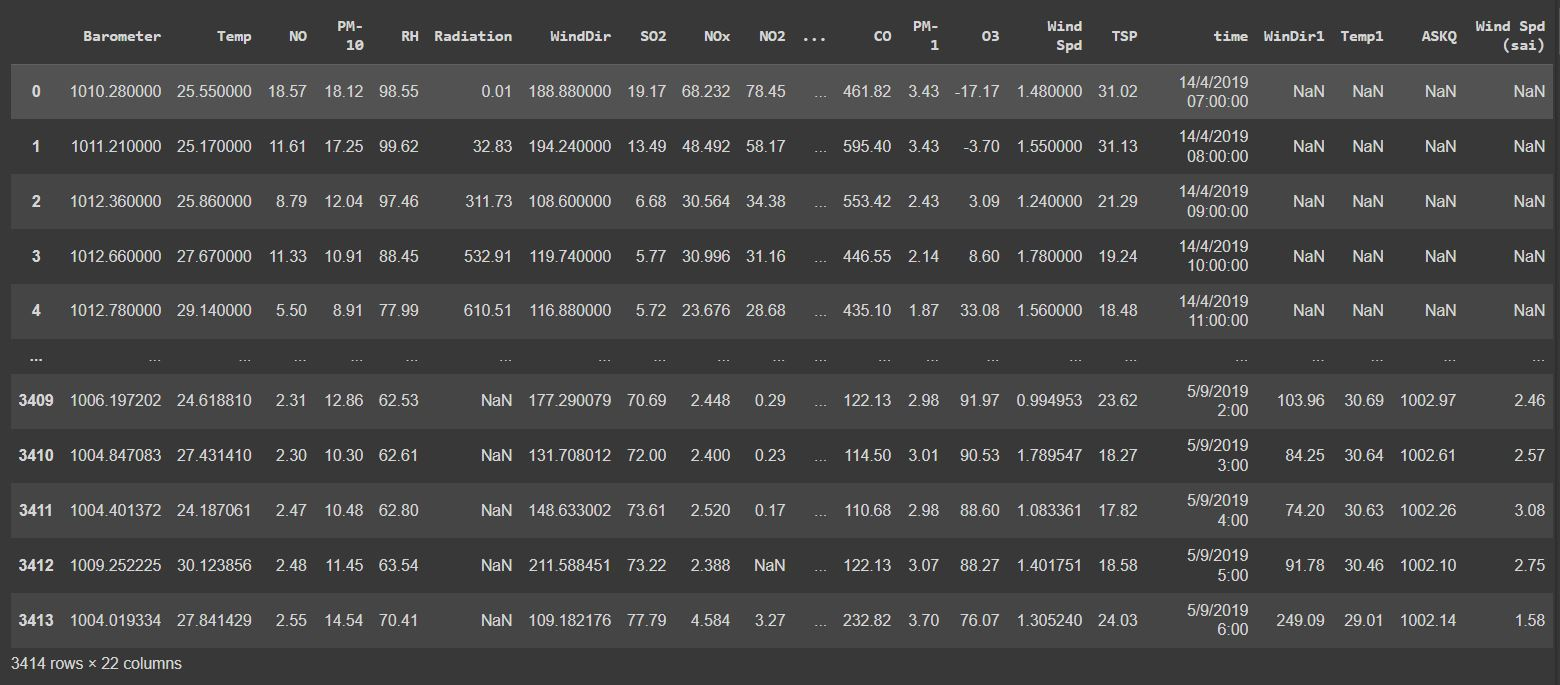
\includegraphics[width=.95\textwidth]{figures/data.jpg}
    \caption[Dữ liệu môi trường không khí từ  7:00 14/4/2019 đến 6:00 5/9/2019]{Dữ liệu môi trường không khí từ  7:00 14/4/2019 đến 6:00 5/9/2019}
\end{figure}
    \end{frame}
\begin{frame}{Tiền xử lý dữ liệu}
\noindent Sử dụng giá trị trung bình của từng cột cho các giá trị còn thiếu ta thu được kết quả:
\begin{figure}[H]
    \centering
    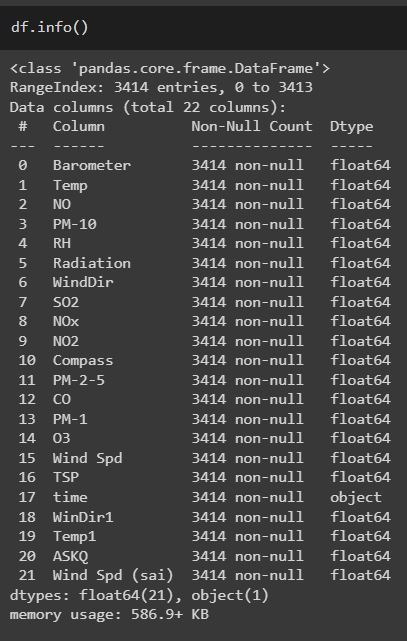
\includegraphics[width=.3\textwidth]{figures/info.jpg}
    \caption[Thông tin dữ liệu sau khi xử lý]{Thông tin dữ liệu sau khi xử lý}
\end{figure}
    \end{frame}
    
    
    
    \begin{frame}{Frame Title}
	\frametitle{Các metrics đánh giá}
    Root Mean Squared Error (RMSE):
    \begin{equation}
    \text{RMSE} = \sqrt{\frac{1}{n}\sum_{i=0}^n(y_i - \hat{y_i})^2}
    \end{equation}
    với $y_i$ là giá trị thực sự cần dự đoán, và $\hat{y}_i$ là giá trị mô hình dự đoán, $n$ là kích thước của dữ liệu cần dự đoán.
    \end{frame}
    
    \begin{frame}{Frame Title}
	\frametitle{Các metrics đánh giá}
Mean Squared Error (MSE):\\
MSE được hiểu là giá trị sai số bình phương trung bình hoặc là lỗi bình phương trung bình. Nó đề cập đến giá trị trung bình của chênh lệch bình phương giữa tham số dự đoán và tham số quan sát được và có công thức như sau:
\begin{equation}
    \text{MSE} = \frac{1}{n}\sum_{i=1}^n(y_i - \hat{y_i})^2
\end{equation}
với $y_i$ là giá trị thực sự cần dự đoán, và $\hat{y}_i$ là giá trị mô hình dự đoán, $n$ là kích thước của dữ liệu cần dự đoán..
    \end{frame}
    
    \begin{frame}{Frame Title}
	\frametitle{Kết quả -LSTM}
    LOSS: được tính bằng MSE, LOSS của mô hình sau khi huấn luyện qua 200 epoch
    \begin{figure}[H]
    \centering
    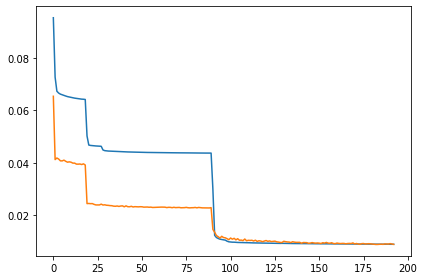
\includegraphics[width=.85\textwidth]{figures/LOSS_LSTM.png}
    \caption[LOSS của mô hình LSTM]{LOSS của mô hình LSTM}
    \end{figure}    
	\end{frame}
	
    \begin{frame}{Frame Title}
	\frametitle{Kết quả}
RMSE của mô hình sau khi huấn luyện qua 200 epoch:
    \begin{figure}[H]
    \centering
    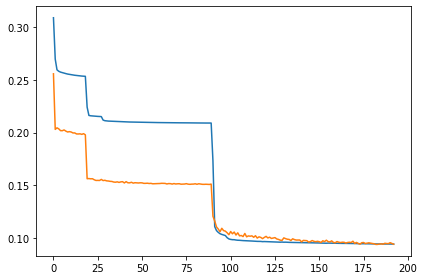
\includegraphics[width=.85\textwidth]{figures/RMSE_LSTM.png}
    \caption[RMSE của mô hình LSTM]{RMSE của mô hình LSTM}
\end{figure}      
	\end{frame}
	
	\begin{frame}{Frame Title}
	\frametitle{Kết quả}
Kết quả dự đoán của mô hình với 48h cuối của bộ dữ liệu so với giá trị thực trên tập dữ liệu, trên một số cột:
\begin{figure}[H]
    \centering
    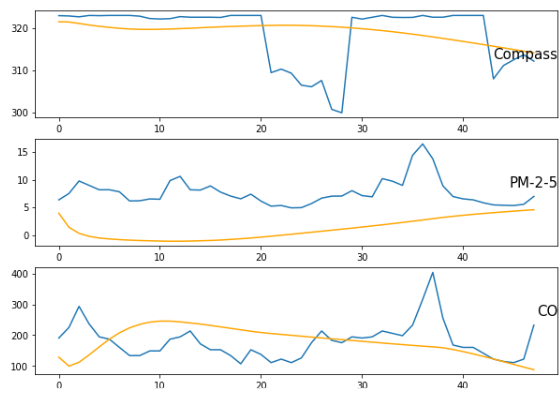
\includegraphics[width=0.7\textwidth]{figures/LSTM_test6.png}
    \caption[Compass, PM-2-5 và CO]{Compass, PM-2-5 và CO}
\end{figure}      
	\end{frame}

\begin{frame}{Frame Title}
	\frametitle{Kết quả -VARMAX}
 \begin{itemize}
     \item Giá trị MSE của mô hình sau khi huấn luyện là \textbf{1031.6635015800691} 
    \item Kết quả đánh giá theo một số cột:
    \begin{figure}[H]
        \centering
        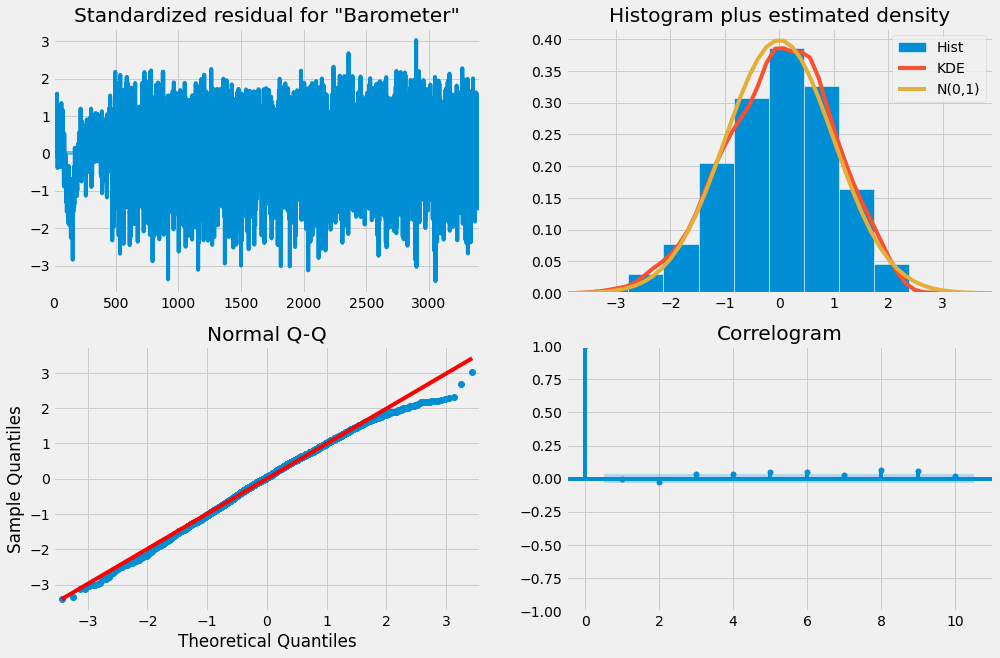
\includegraphics[width=0.6\textwidth]{figures/danhgia1.png}
        \caption[Barometer]{Barometer}
    \end{figure}
    \end{itemize}
	\end{frame}

  \begin{frame}{Frame Title}
	\frametitle{Kết quả }
 
    \begin{figure}[H]
        \centering
        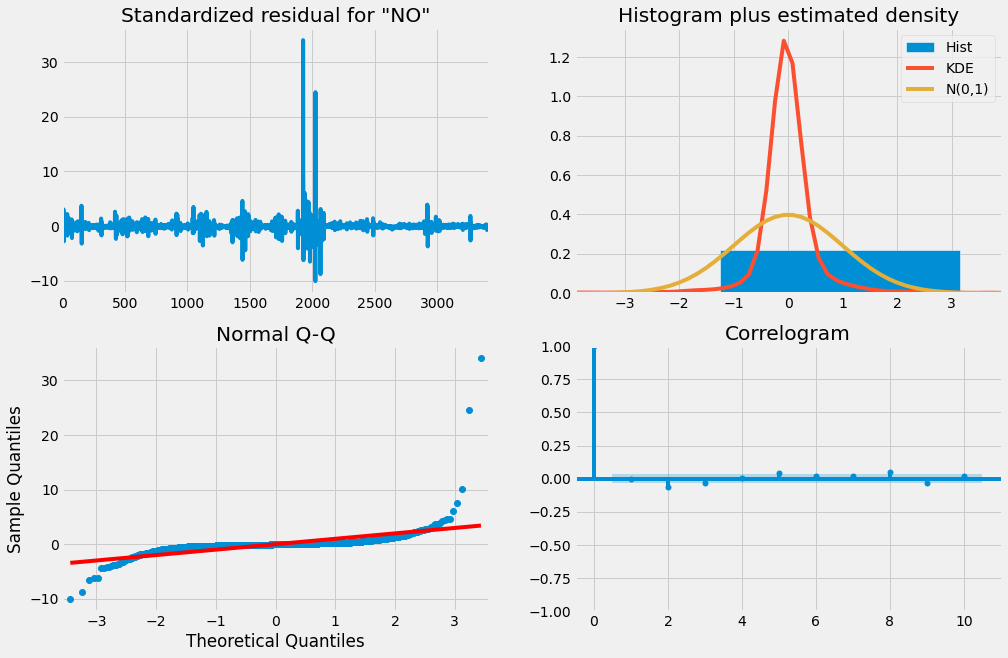
\includegraphics[width=0.6\textwidth]{figures/danhgia3.png}
        \caption[NO]{NO}
    \end{figure}
	\end{frame}	
 \begin{frame}{Frame Title}
	\frametitle{Kết quả }
 
    Kết quả dự đoán so với tập test
    \begin{figure}[H]
        \centering
        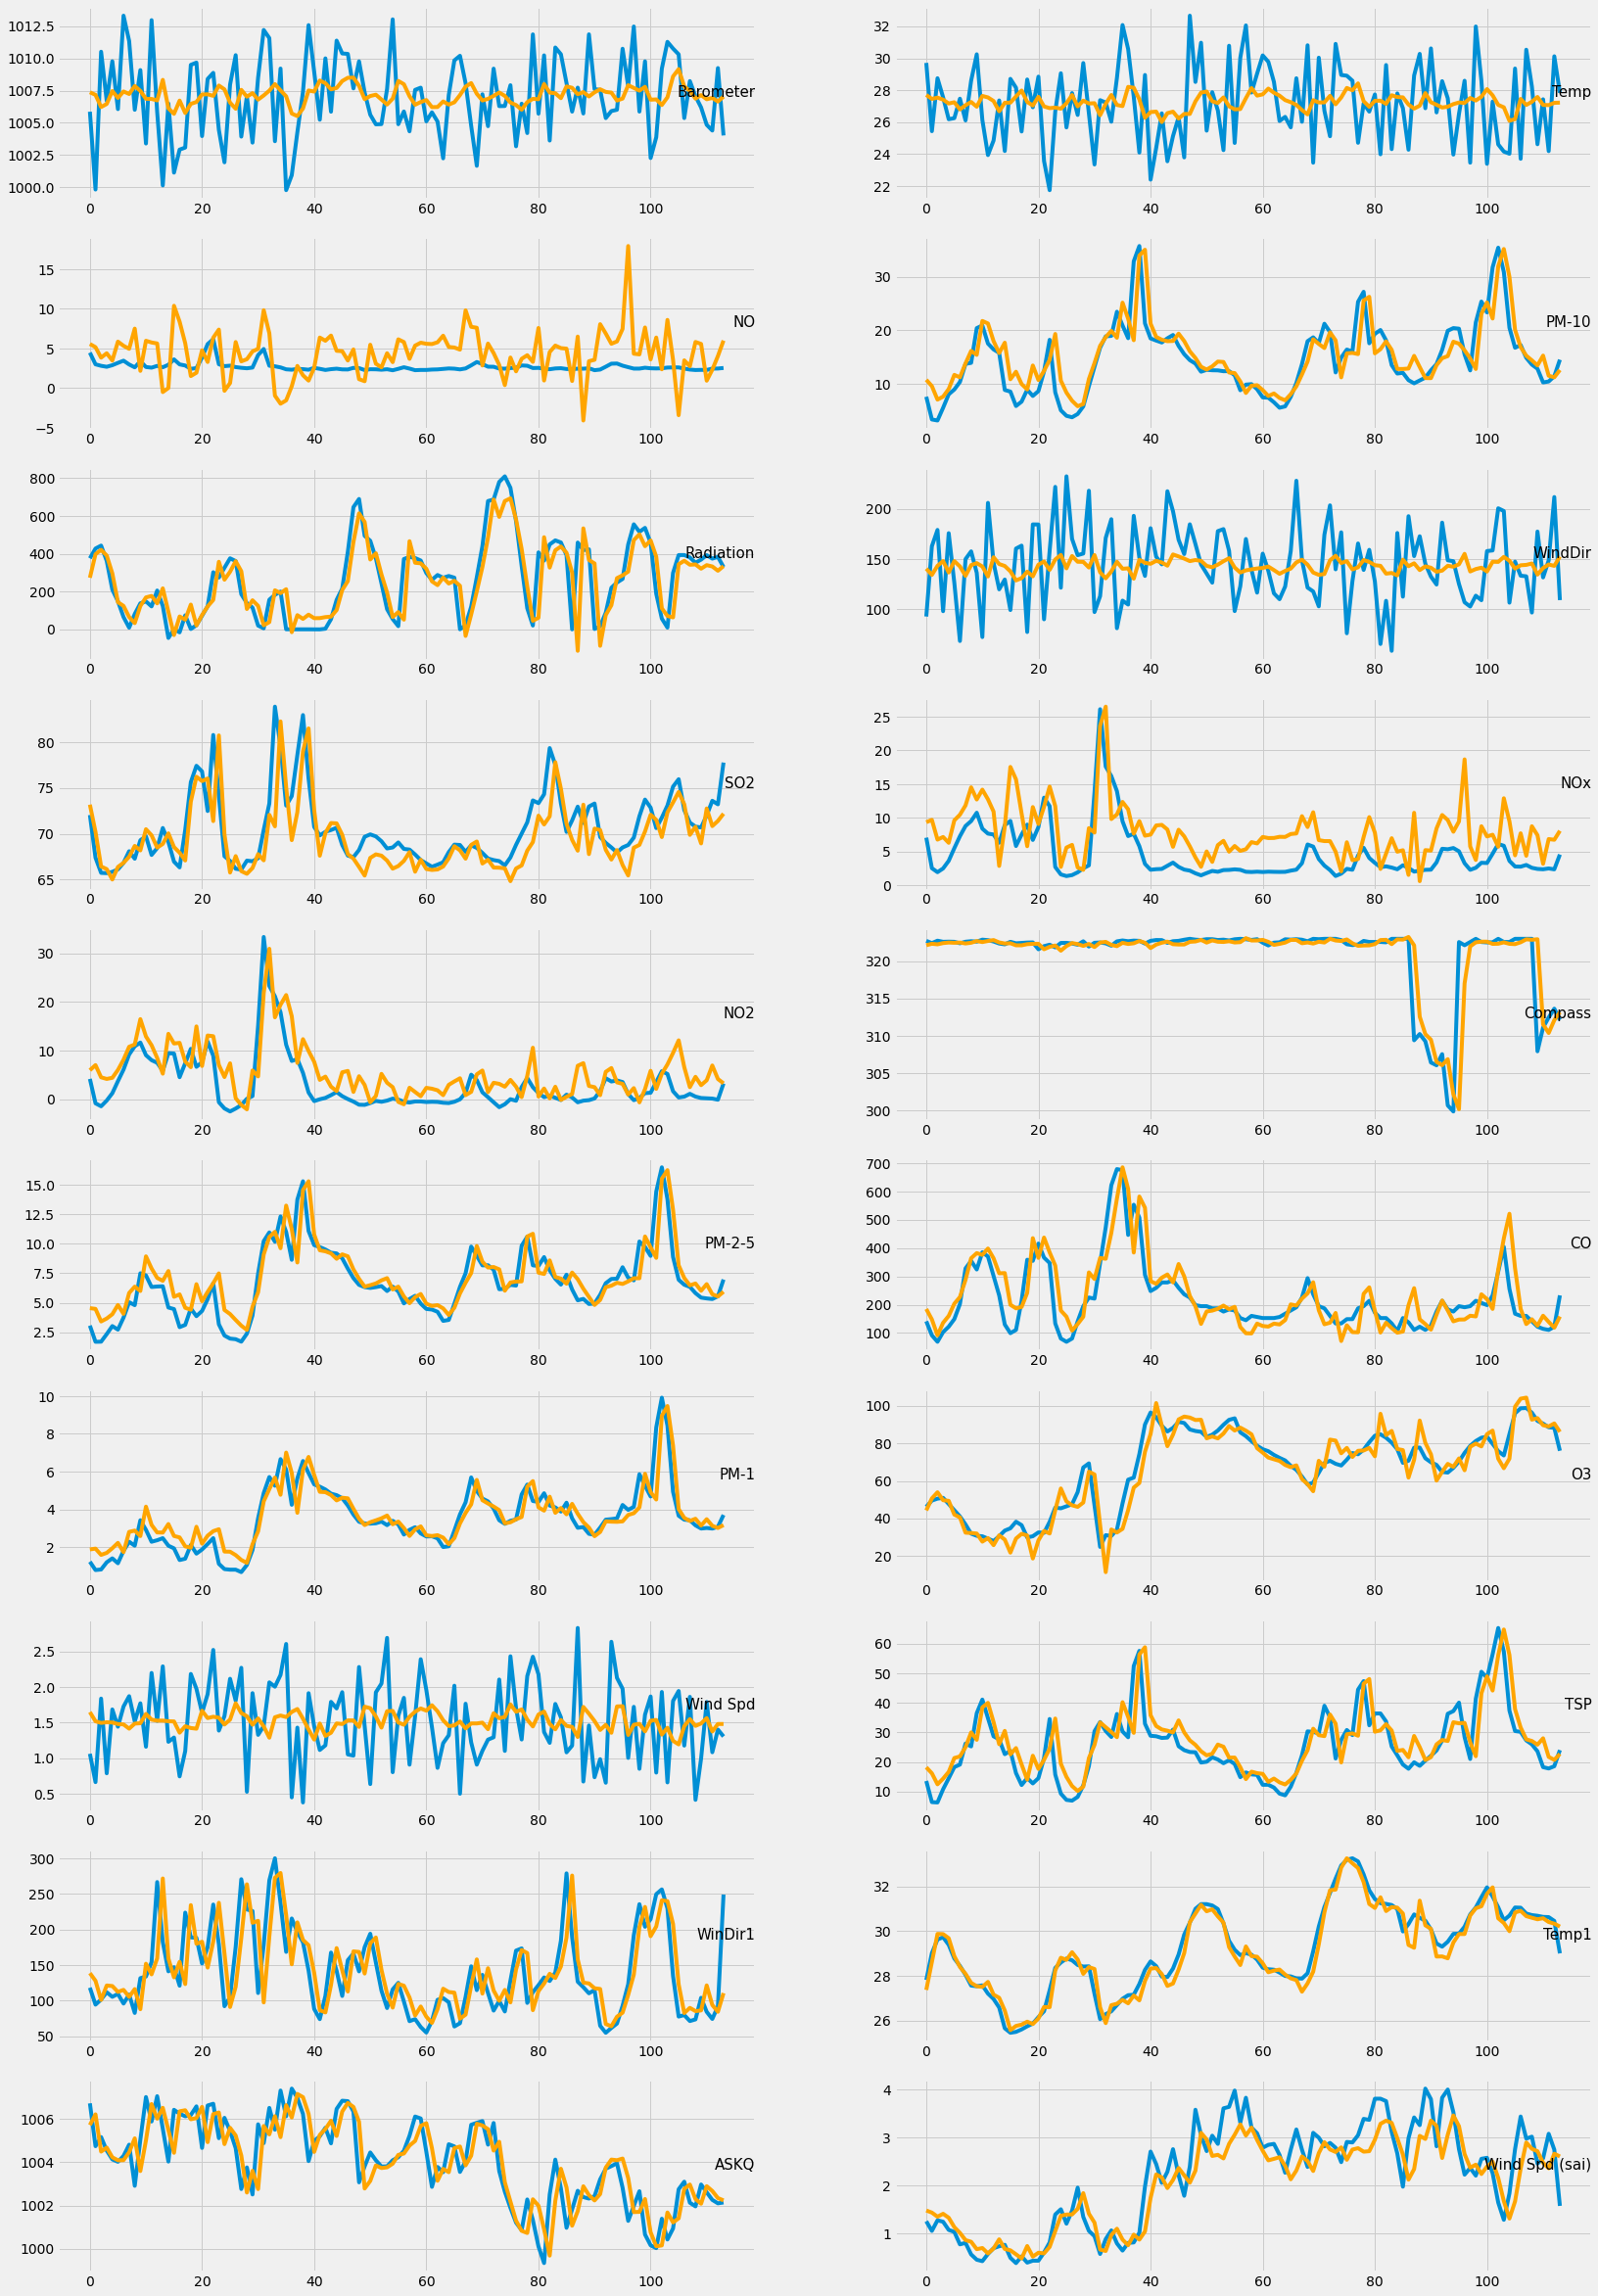
\includegraphics[width=.35\textwidth]{figures/VAR_test.png}
        \caption[Kết quả dự đoán so với tập test]{Kết quả dự đoán so với tập test}
    \end{figure}
	\end{frame}	
 %\begin{frame}{Frame Title}
%	\frametitle{Kết quả }
 
%    Kết quả dự đoán 48 giờ sau đó
%    \begin{figure}[H]
%        \centering
%        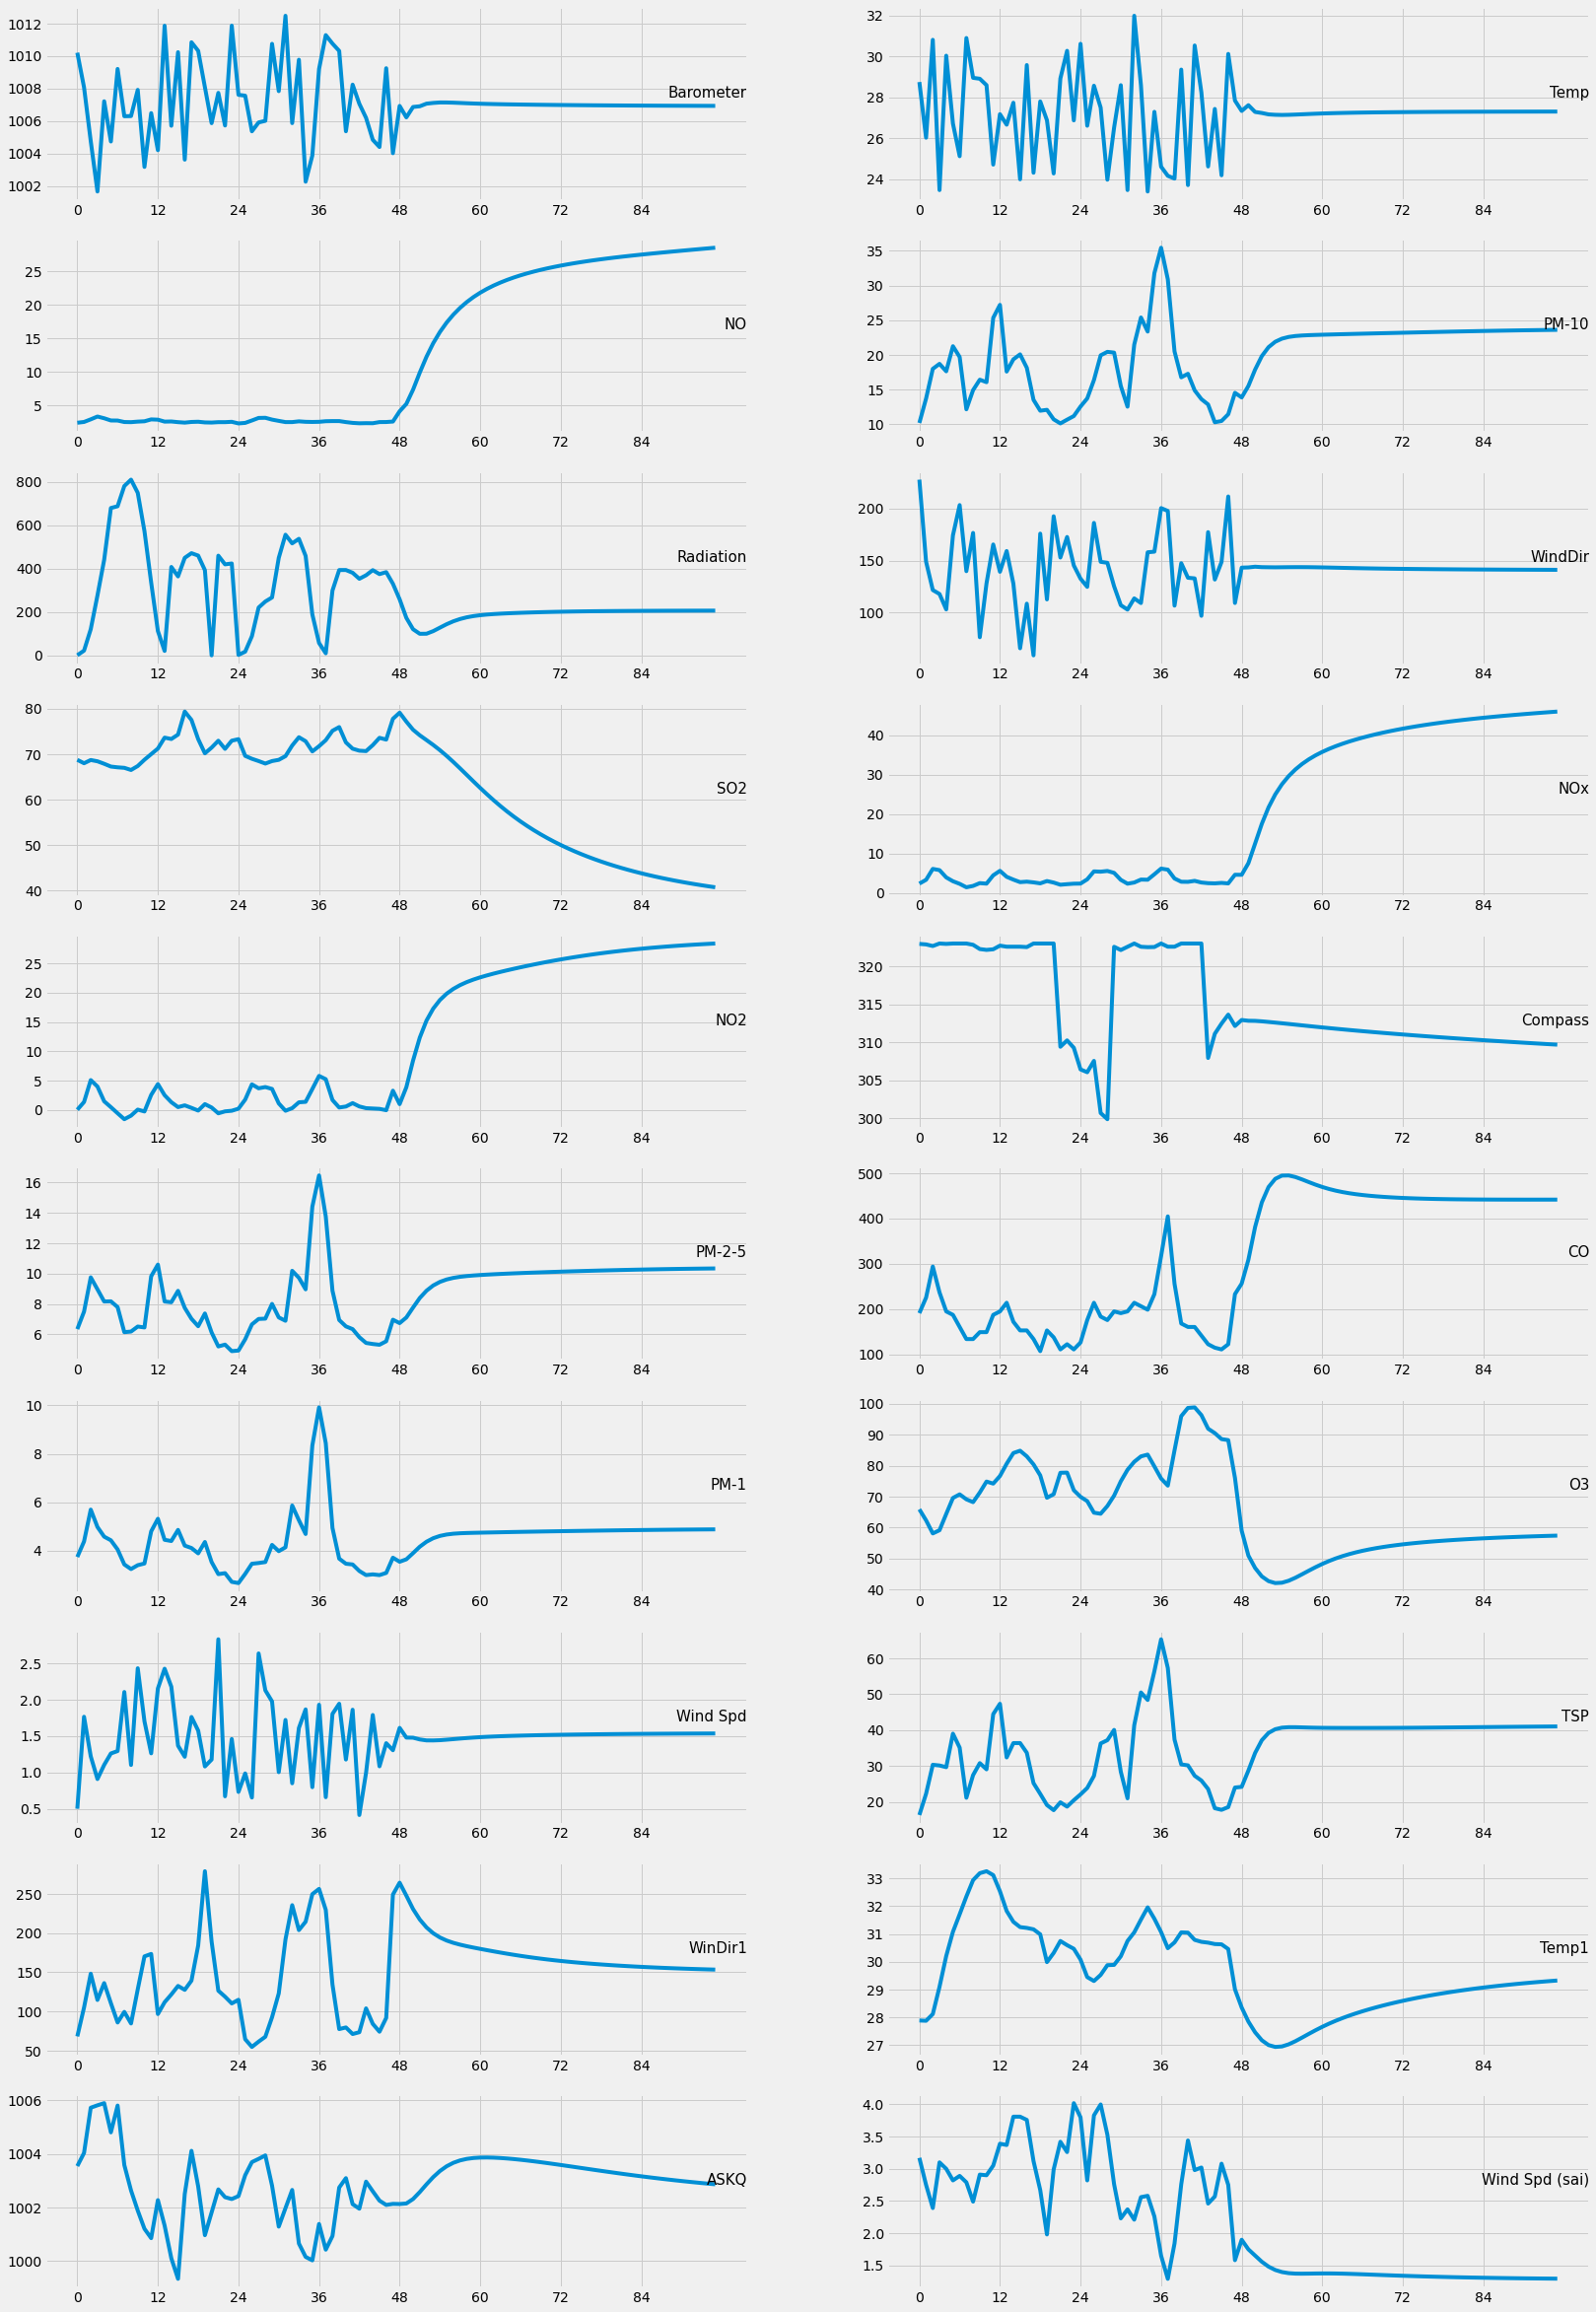
\includegraphics[width=.35\textwidth]{figures/VAR_predic.png}
%        \caption[Kết quả dự đoán 48 giờ sau đó]{Kết quả dự đoán 48h sau đó}
%    \end{figure}
%	\end{frame}	

 
 
	\section{Kết luận}
	\begin{frame}{Những điều đã làm được}
	    Trong phạm vi nội dung của bài tập lớn, một số nội dung mà nhóm chúng em đã đạt được:
\begin{itemize}
    \item Thành công trong việc giới thiệu 2 mô hình dự đoán chuỗi thời gian VARMAX và LSTM. 
    \item Ứng dụng được vào bài toán dự đoán chất lượng không khí.
\end{itemize}
	\end{frame}

\end{footnotesize}
\begin{frame}{}
\centering
    \Huge{\textbf{Thanks for listening!}}
\end{frame}
\bibliographystyle{plain}
\bibliography{References.bib}   


\end{document}